\documentclass[11pt]{article}

\usepackage[margin=1in]{geometry}
\IfFileExists{lmodern.sty}{\usepackage[T1]{fontenc}\usepackage{lmodern}}{}
\usepackage{microtype}
\usepackage{amsmath,amssymb,amsthm,mathtools}
\usepackage{booktabs}
\usepackage{graphicx}
\usepackage{caption}
\usepackage{enumitem}
\usepackage[authoryear,round]{natbib}
\usepackage{xcolor}
\usepackage[section]{placeins}
\usepackage[colorlinks=true,linkcolor=blue!50!black,citecolor=blue!50!black,urlcolor=blue!50!black]{hyperref}

\graphicspath{{../results/figures/}}
\newcommand{\tablefile}[1]{\input{../results/tables/#1}}

\newtheorem{assumption}{Assumption}
\newtheorem{proposition}{Proposition}
\newtheorem{corollary}{Corollary}
\theoremstyle{remark}
\newtheorem{remark}{Remark}

\DeclareMathOperator{\E}{\mathbb{E}}
\newcommand{\Prob}{\mathbb{P}}
\newcommand{\indep}{\perp\!\!\!\perp}
\newcommand{\1}{\mathbf{1}}
\newcommand{\cX}{\mathcal{X}}
\newcommand{\cD}{\mathcal{D}}
\newcommand{\cA}{\mathcal{A}}
\newcommand{\cB}{\mathcal{B}}
\newcommand{\cC}{\mathcal{C}}
\newcommand{\cN}{\mathcal{N}}

\captionsetup{font=small,labelfont=bf}
\setlength{\parskip}{0.35em}

\begin{document}

\begin{titlepage}
  \centering
  \vspace*{2.5cm}
  {\LARGE\bfseries Bounds on the Dynamic Causal Effects\\[4pt] of Monetary Policy\par}
  \vspace{0.6cm}
  {\large An Analysis Using the Federal Reserve's Textual Repository\par}
  \vspace{2cm}
  {\Large Felipe Pombal Fritsch\par}
  \vspace{0.6cm}
  {\large Advisor: Prof.\ Jos\'e Luis Montiel Olea\par}
  \vfill
  A thesis presented for the degree of Bachelor of Arts\\
  Department of Economics, Columbia University\\[1em]
  Submitted May 2020 \quad$\cdot$\quad Revised edition, September 2026
\end{titlepage}

\begin{abstract}
\noindent
Semiparametric estimates of the effects of monetary policy treat each FOMC meeting as a unit that selects into a
policy choice, and require every choice to be possible at every point of the covariate space (overlap). Using the
policy alternatives that Federal Reserve staff lay out in the Bluebook before each meeting, I show that overlap
fails in a specific, observable way: over 133 meetings from 1989 to 2006 the Committee never took an action that
was absent from its menu. I build a propensity-score model in which the menu imposes these structural zeros,
derive the sharp identified set for the average dynamic effect of a rate increase or decrease when some menus
exclude the action or the status quo, and propose a one-parameter relaxation that trades the worst case for an
assumption on effect heterogeneity across menus. The menu constraint alone improves the fit of the policy
model as much as adding market expectations. On the empirical side, worst-case bounds are uninformative, and the
effects that are point-identified on the meetings with genuine overlap have the wrong sign for industrial
production and unemployment even after conditioning on the Greenbook forecasts, although the forecasts do remove
the price puzzle. Handling overlap does not rescue selection-on-observables in this setting: the binding problem is
unconfoundedness.
\end{abstract}

\vspace{1em}
\noindent\fbox{\parbox{\dimexpr\linewidth-2\fboxsep-2\fboxrule}{\small
\textbf{Note on this edition.} This revision replaces the version submitted in May 2020. The conceptual idea is
unchanged; the estimation was revised and the code rebuilt from the raw data. The main changes are the propensity
score, the calibration of the outcome bounds, the treatment of the point estimates, and the addition of inference.
Several conclusions change as a result. Appendix~\ref{app:revision} compares the two versions. All numbers here are
produced by the pipeline in the accompanying repository.}}

\newpage
\tableofcontents
\newpage

\section{Introduction}\label{sec:intro}

Measuring the effect of monetary policy on the economy is one of the central problems of empirical
macroeconomics. The difficulty is familiar. Policy responds to the state of the economy, which in turn responds to
policy, and the econometrician sees a few hundred monthly observations of this feedback loop. The dominant
response has been to impose structure, through structural vector autoregressions \citep{sims1980} or local
projections \citep{jorda2005}, and with it linearity in the effect of policy.

A second approach, developed by \citet{angrist2011} and \citet{angrist2018}, borrows from microeconometric policy
evaluation. Each FOMC meeting is a unit that selects into a policy choice (ease, hold, or tighten), and the
effect of that choice is recovered by inverse probability weighting (IPW) on a propensity score for the
Committee's decision. The approach is semiparametric and allows effects to be nonlinear and asymmetric. Like all
selection-on-observables designs, however, it rests on two assumptions. \emph{Unconfoundedness} requires that,
given the observed covariates, the decision be unrelated to the future path the economy would take under each
alternative. \emph{Overlap} requires every decision to have positive probability at every value of the covariates.

This thesis starts from the second assumption. Some policy actions are simply not on the table in some states
of the economy. The Federal Reserve's own documents record which: before every meeting, Board staff circulate the
Bluebook, which lists the policy alternatives the Committee will consider. I use these \emph{policy menus},
extracted from the Bluebooks by text analysis, to make three contributions.
\begin{enumerate}[leftmargin=*,itemsep=2pt]
  \item \textbf{Structural non-overlap is observable.} In 133 scheduled meetings between August 1989 and
  January 2006 the FOMC never chose an action that was not on its Bluebook menu, and two thirds of the menus exclude
  either easing or tightening. The failure of overlap is not a feature of a fitted model. It is recorded in
  the Committee's briefing documents.
  \item \textbf{Menu-constrained propensity score and sharp bounds.} I estimate the decision model as an
  ordered probit renormalised over the menu, so that the propensity score is exactly zero for an action that is
  not on the menu. I then derive the sharp identified set for the average effect of a rate increase or decrease,
  exploiting the fact that in a menu that contains the status quo but not the action (or the reverse) half of
  the comparison is still identified. A one-parameter relaxation bounds how far effects in the non-overlap menus
  may differ from the effect in the overlap region, and yields a breakdown value for each estimate's sign.
  \item \textbf{Evidence.} Imposing the menus raises the log likelihood of the decision model by almost 19 points
  without any additional parameters. However, the effects that are point-identified on the overlap region imply that
  rate increases are followed by higher industrial production and lower unemployment, even when the propensity
  score conditions on the Greenbook forecasts that \citet{romer2004} use to purge policy of its predictable
  component. Worst-case bounds that make no assumption on the missing menus are wide and contain zero.
\end{enumerate}

The negative result is informative. It shows that correcting the overlap problem, which is real and
documented, does not deliver credible effects of monetary policy under selection on observables in this sample:
what remains is a failure of unconfoundedness, most plausibly because the Committee acts on information about the
future economy that neither macro aggregates, market expectations nor staff forecasts fully capture. The bounds
framework makes this transparent, because it separates what the data identify from what must be assumed.

\paragraph{Related literature.} The potential-outcomes approach to monetary policy follows \citet{angrist2011},
\citet{angrist2018} and \citet{rambachan2019}. The consequences of limited overlap for IPW are studied by
\citet{khan2010}, \citet{crump2009}, \citet{ma2020} and, with many covariates, \citet{damour2021}; I study the
case in which overlap fails exactly and the region of failure is observed. The bounds follow \citet{manski1990,manski2003},
and inference follows \citet{imbens2004}. The text data build on the FOMC text-analysis project of Montiel Olea and
coauthors and relate to \citet{hansen2018}. The use of staff forecasts to control for the Federal Reserve's
information set follows \citet{romer2004}.

\paragraph{Outline.} Section~\ref{sec:data} describes the FOMC's decision process and the construction of the
policy menus. Section~\ref{sec:framework} sets out the framework and derives the bounds. Section~\ref{sec:estimation}
covers estimation and inference, and Section~\ref{sec:results} reports results. Section~\ref{sec:conclusion} concludes.

\section{Related Literature}\label{sec:literature}

This thesis sits where four literatures meet: the potential-outcomes approach to dynamic causal effects in
macroeconomics, the identification of monetary policy shocks, the use of the Federal Reserve's text as data, and
the econometrics of weighting estimators when overlap is limited or fails. Each has moved substantially since the
first version of this thesis was written in 2020.

\subsection{Dynamic causal effects and potential outcomes}

\citet{angrist2011} and \citet{angrist2018} recast the effect of monetary policy as a policy-evaluation problem:
each FOMC decision is a treatment, a propensity score for the Committee's choice is estimated by ordered probit,
and impulse responses are inverse-probability-weighted averages of future outcomes. Their approach is robust to
nonlinearity and asymmetry, and it requires selection on observables and overlap. \citet{rambachan2025} give the
general framework: a ``direct potential outcome system'' in which impulse responses and local projections have a
nonparametric causal interpretation under conditions they make precise. This thesis adopts their notation for
potential outcomes indexed by the policy action and the horizon.

A closely related line asks what the standard linear tools estimate when the world is not linear.
\citet{plagborg2021} show that local projections and VARs estimate the same population impulse responses, so the
choice between them is about finite-sample bias and variance, not about the estimand. \citet{kolesar2025} show that
VARs and linear local projections on an observed shock or proxy identify \emph{weighted averages} of causal effects
however nonlinear the data-generating process, whereas methods that rely on heteroskedasticity or non-Gaussianity
for identification can fail. The IPW estimator used here targets an unweighted average effect of a discrete policy
action instead. The price is that it needs a correctly specified propensity score and, as this thesis emphasises,
overlap. \citet{montielolea2021} show that lag-augmented local projections give valid inference even with persistent
data and at long horizons. Their result is a useful benchmark for the inference problem this thesis faces, in which
outcomes at nearby meetings overlap in time.

\subsection{Identifying monetary policy shocks and the Federal Reserve's information}

The central difficulty in estimating the effect of monetary policy is that the Federal Reserve reacts to what it
expects the economy to do. \citet{romer2004} addressed this by purging the intended funds-rate change of its
response to the Greenbook forecasts. \citet{romer2023} revisit thirty-five years of narrative evidence and argue
that carefully identified shocks have large effects on output, unemployment and inflation in the expected
directions. High-frequency identification uses the change in market rates in a narrow window around FOMC
announcements instead. \citet{nakamura2018} argue that such surprises also reveal the Fed's private information
about the economy (an ``information effect''), and \citet{jarocinski2020} and \citet{mirandaagrippino2021}
separate pure policy shocks from information shocks using the joint response of stock prices or private forecasts.
\citet{bauer2023aer,bauer2023nber} offer an alternative account: much of the apparent information effect reflects
the Fed responding to economic news that markets had not yet priced, which makes raw surprises predictable and
calls for orthogonalising them with respect to prior news.

Most closely related to this thesis, \citet{aruoba2025} use natural language processing on the staff documents
prepared before each FOMC meeting to measure the Committee's information set. They find that the text contains
information about the economy that the Greenbook's numerical forecasts do not, and that shocks identified as
residuals from a model that uses it produce responses consistent with standard theory. Their conclusion speaks
directly to the empirical results of Section~\ref{sec:results}: conditioning on numerical forecasts alone may leave
enough of the Fed's information out of the propensity score to bias selection-on-observables estimates.

\subsection{The Federal Reserve's text as data}

\citet{hansen2018} brought computational linguistics to the FOMC transcripts, and the use of the Fed's internal
documents has since grown quickly. \citet{ke2022} develop robust topic-model estimators and apply them to the
transcripts of the Greenspan era, the period studied here. Two recent papers use the Bluebook alternatives
themselves. \citet{doh2026} fine-tune a language model on the alternative policy statements drafted by Board staff
to measure where the adopted statement sits on the dovish--hawkish spectrum, and \citet{laarits2025} use the
alternatives circulated before each meeting to study how the Committee aggregates members' differing economic
models. This thesis uses the same documents for a different purpose: not to measure the tone of communication, but
to recover the set of actions the Committee considered, which determines where the propensity score is zero.

\subsection{Overlap, weighting and partial identification}

When propensity scores approach zero, IPW estimators become unstable and standard inference can fail.
\citet{khan2010} show that identification is then irregular and convergence slower than $\sqrt{n}$;
\citet{crump2009} propose trimming to a subpopulation with good overlap; \citet{ma2020} and \citet{heiler2021}
develop inference that remains valid with small or many extreme scores; and \citet{damour2021} show that strict
overlap becomes restrictive when there are many covariates. All of these treat limited overlap as a feature of the
estimated score. The distinguishing feature of the present setting is that overlap fails \emph{exactly}, and the
region where it fails is recorded in the data.

For that case, partial identification is the natural tool. Worst-case bounds under a support restriction go back to
\citet{manski1990,manski2003}, and \citet{imbens2004} give confidence intervals for the partially identified
parameter. \citet{susmann2025} develop bounds on the average treatment effect in the cross-sectional setting when
outcome overlap fails for a subpopulation, with width equal to the outcome range times the probability of that
subpopulation, and propose efficient estimators and uniformly valid inference. Proposition~\ref{prop:bounds}
is the analogue for a multi-valued treatment in a time series, where the non-overlap region is observed rather than
estimated and some menus contain only one of the two actions being compared. Finally, a large literature relaxes
unconfoundedness itself; \citet{masten2018} bound treatment effects when selection on unobservables is limited by a
sensitivity parameter, an approach that complements the $\lambda$-relaxation of Section~\ref{sec:framework}, which
relaxes effect homogeneity across menus instead.

\section{Data: Policy Menus from the Bluebooks}\label{sec:data}

\subsection{How the FOMC prepares a decision}

The Federal Open Market Committee (FOMC) meets eight times a year at scheduled meetings and occasionally by
conference call. Each scheduled meeting is preceded by a structured set of staff documents
\citep{danker2005}. About two weeks before the meeting the \emph{Beige Book} summarises anecdotal evidence from
the twelve Reserve Bank districts. About a week before, the \emph{Greenbook} gives the Board staff's forecast for
the domestic and international economy. On the Friday before the meeting the \emph{Bluebook} sets out the policy
alternatives for the Committee's consideration, usually labelled A, B and C, each with a proposed federal funds
rate target and a rationale. The meeting agenda then includes a discussion of these alternatives before the
Committee votes. The format of these documents has changed over time: documents have been introduced, merged and
retired since the corpus begins in 1936. Over the sample used here the sequence above is stable.

Two of these documents enter the analysis. The Bluebook defines the \emph{menu} of actions the Committee
considered, which is the object of this thesis, and the Greenbook provides the staff forecasts used as
covariates in Section~\ref{sec:estimation}.

\subsection{Extracting the menus}

The Bluebooks are published with a five-year lag on the Board's website as HTML and PDF files. Building on the
FOMC text-analysis project of Montiel Olea, Giesecke, Chitale and Frermann, the documents were converted to raw
text and every sentence mentioning a policy alternative was extracted with the regular expression
\begin{center}
\small\verb/([^.]*)(alternatives?\s+[a-e])(\.|[^a-z]\.|[^a-z][^\.]+\.)/
\end{center}
which captures a sentence containing ``alternative'' followed by a letter. The extracted sentences were then
read and classified by hand, because the same target is sometimes described in different ways under different
rationales. For each alternative I record the proposed change in the federal funds rate target, and classify it
as easing ($E$), unchanged ($U$) or tightening ($T$).

The Committee's actual decision is taken from the target changes in the replication files of
\citet{angrist2018}. The sample runs from August 1989 to January 2006, the Greenspan chairmanship after the
Committee had begun to target the federal funds rate explicitly \citep{romer2004}. It contains 133 scheduled
meetings with a Bluebook menu. Target changes of 25, 50 and 75 basis points are pooled into the three categories
because 50 and 75 basis point moves are too rare to estimate separately.

\subsection{What the menus show}

Table~\ref{tab:menus} cross-tabulates the menu offered with the decision taken. Two facts stand out. First, the
decision is \emph{always} on the menu: no meeting in the sample took an action that the Bluebook did not propose.
The zeros in Table~\ref{tab:menus} are therefore structural, and they are observed rather than inferred. Second, most
menus are restricted: 87 of 133 meetings (65\%) were offered a menu without easing or without tightening, and only
46 had all three options. The full menu is also where the Committee was least likely to move. Only one of the 27
tightenings in the sample came from a full menu.

\begin{table}[!htbp]
  \centering
  \caption{Bluebook menus and FOMC decisions, August 1989 -- January 2006}\label{tab:menus}
  \tablefile{menus.tex}
  \par\medskip
  \begin{minipage}{0.8\linewidth}\footnotesize
  \emph{Notes:} Scheduled FOMC meetings. Rows give the set of alternatives proposed in the Bluebook ($E$ ease,
  $U$ unchanged, $T$ tighten); columns give the decision. Every decision lies in the menu.
  \end{minipage}
\end{table}

Figure~\ref{fig:state} shows where in the macroeconomic state space these restrictions bind. Panel (a) plots
lagged inflation and industrial-production growth at each meeting, marking the meetings at which the Committee
tightened or eased. Panel (b) marks instead the meetings whose menu \emph{excluded} easing or tightening. Menus
without easing are concentrated where output growth is above its sample average (88\% of them), and menus without
tightening where it is below (78\%). The same pattern appears in the decisions themselves, but the menu shows it
without relying on a fitted model: in about half of the meetings with below-average output growth (29 of 56) tightening
was not even proposed, and the Committee tightened at only three of them. This is
exactly the kind of covariate region in which a propensity score must be zero, and it is why a standard IPW
estimator, which divides by the propensity score, is not available there.

\begin{figure}[!htbp]
  \centering
  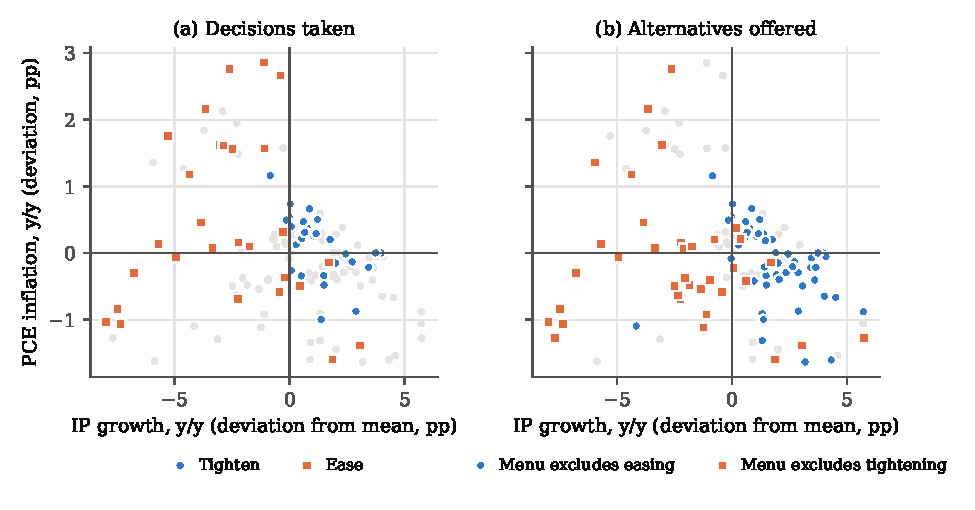
\includegraphics[width=\linewidth]{state_space.pdf}
  \caption{Policy decisions and policy menus in the inflation--output space. Each point is a scheduled FOMC
  meeting; axes show year-on-year PCE inflation and industrial-production growth in the previous month, as
  deviations from their 1989--2006 means. Grey points are meetings not in the highlighted group.}\label{fig:state}
\end{figure}

\section{Framework: Policy Evaluation When Overlap Fails by Design}\label{sec:framework}

\subsection{Treatment, menus and potential outcomes}

Index scheduled FOMC meetings by $t$. The policy decision is $D_t\in\cD=\{-1,0,1\}$ (ease, leave unchanged,
tighten the federal funds rate target). The Bluebook menu is $X_t\in\cX$, a non-empty subset of $\cD$; in the data
$\cX=\{\{-1\},\{0\},\{1\},\{-1,0\},\{0,1\},\{-1,0,1\}\}$. Other information available to the Committee (lagged
macroeconomic data, market expectations, staff forecasts) is collected in $Z_t\in\mathbb{R}^k$, and
$W_t=(X_t,Z_t)$.

For an outcome series $y$ (log industrial production, the unemployment rate, the log PCE price index), let
$Y_{t,h}=y_{t+h}-y_t$ be its cumulative change over the $h$ months following the meeting. Each decision $d$
induces a potential outcome $Y_{t,h}(d)$, and $Y_{t,h}=\sum_{d\in\cD}\1\{D_t=d\}\,Y_{t,h}(d)$. The parameter of
interest is the average dynamic effect of an increase ($d=1$) or a decrease ($d=-1$) relative to leaving the target
unchanged,
\begin{equation}\label{eq:theta}
  \theta_d(h)=\E\bigl[Y_{t,h}(d)-Y_{t,h}(0)\bigr],\qquad d\in\{-1,1\},\ h=1,\dots,24 .
\end{equation}
Expectations are taken over the stationary distribution of meetings. I drop the $t$ and $h$ subscripts when they
are not needed. The propensity score is $p_d(w)=\Prob(D=d\mid W=w)$.

\subsection{Assumptions}

\begin{assumption}[Selection on observables]\label{as:unconf}
$Y_{h}(d)\indep D\mid W$ for all $d\in\cD$ and all $h$.
\end{assumption}

\begin{assumption}[Menu overlap]\label{as:menu}
For all $w=(x,z)$ in the support of $W$: $p_d(x,z)>0$ if and only if $d\in x$.
\end{assumption}

\begin{assumption}[Bounded outcomes]\label{as:bounded}
$Y_{h}(d)\in[K_{1h},K_{2h}]$ almost surely, for all $d$ and $h$, with known $K_{1h}<K_{2h}$.
\end{assumption}

Assumption~\ref{as:unconf} is the identifying assumption of \citet{angrist2018}. It says that once we condition
on what the Committee knew, including what it was offered, the remaining variation in its decision is as good as
random with respect to the economy's future path. Assumption~\ref{as:menu} replaces the usual overlap condition,
$p_d(w)>0$ for all $d$ and $w$. It allows the propensity score to be zero, but only in the way the Bluebook
dictates: the Committee does not take an action that is not on the menu (which holds without exception in the
data, Table~\ref{tab:menus}), and any action on the menu has some chance of being taken. The ``only if'' part is
testable and holds. The ``if'' part is an assumption. Assumption~\ref{as:bounded} is a support restriction of
the kind used by \citet{manski1990}. It bites only on the cells in which the data are silent.

\subsection{What the data identify}

Write $\pi_x=\Prob(X=x)$ and $\mu_d(x)=\E[Y(d)\mid X=x]$. Conditioning on the menu,
\begin{equation}\label{eq:decomp}
  \theta_d=\sum_{x\in\cX}\pi_x\,\bigl(\mu_d(x)-\mu_0(x)\bigr).
\end{equation}
Under Assumptions~\ref{as:unconf}--\ref{as:menu}, for any $a\in x$ the conditional mean $\mu_a(x)$ is identified by
inverse probability weighting within the menu:
\begin{equation}\label{eq:ipw}
  \mu_a(x)=\E\!\left[\frac{\1\{D=a\}\,Y}{p_a(X,Z)}\ \middle|\ X=x\right],\qquad a\in x,
\end{equation}
because $p_a(x,Z)>0$ for every $Z$ when $a\in x$. When $a\notin x$, the data never show $Y(a)$ in menu $x$ and
$\mu_a(x)$ is not identified. For a given $d$, partition the menus into four groups:
\begin{align*}
\cA_d&=\{x:\,d\in x,\,0\in x\}, & \cB_d&=\{x:\,0\in x,\,d\notin x\},\\
\cC_d&=\{x:\,d\in x,\,0\notin x\}, & \cN_d&=\{x:\,d\notin x,\,0\notin x\}.
\end{align*}
For $d=1$ these are $\cA_1=\{\{0,1\},\{-1,0,1\}\}$, $\cB_1=\{\{0\},\{-1,0\}\}$, $\cC_1=\{\{1\}\}$ and
$\cN_1=\{\{-1\}\}$. The overlap region $\cA_d$ is where the effect is point-identified. In $\cB_d$ the status-quo mean
is identified but the treated mean is not; in $\cC_d$ the reverse; in $\cN_d$ neither.

\begin{proposition}[Sharp identified set]\label{prop:bounds}
Under Assumptions~\ref{as:unconf}--\ref{as:bounded}, the identified set for $\theta_d(h)$ is the interval
$[L_d,U_d]$ with
\begin{align*}
L_d&=\sum_{x\in\cA_d}\pi_x\bigl(\mu_d(x)-\mu_0(x)\bigr)+\sum_{x\in\cB_d}\pi_x\bigl(K_1-\mu_0(x)\bigr)\\
&\qquad+\sum_{x\in\cC_d}\pi_x\bigl(\mu_d(x)-K_2\bigr)+\sum_{x\in\cN_d}\pi_x\,(K_1-K_2),\\
U_d&=\sum_{x\in\cA_d}\pi_x\bigl(\mu_d(x)-\mu_0(x)\bigr)+\sum_{x\in\cB_d}\pi_x\bigl(K_2-\mu_0(x)\bigr)\\
&\qquad+\sum_{x\in\cC_d}\pi_x\bigl(\mu_d(x)-K_1\bigr)+\sum_{x\in\cN_d}\pi_x\,(K_2-K_1).
\end{align*}
Its width is $U_d-L_d=(K_2-K_1)\bigl[\pi(\cB_d)+\pi(\cC_d)+2\,\pi(\cN_d)\bigr]$.
\end{proposition}

The proof is in Appendix~\ref{app:proofs}. The width is always below the width of the no-information bound,
$2(K_2-K_1)$, so the set is informative whenever some menu contains both $d$ and $0$ or one of them. It is also
narrower than the naive bound that treats every cell outside $\cA_d$ as uninformative, whose width is
$2(K_2-K_1)\bigl[1-\pi(\cA_d)\bigr]$, because the identified half of each one-sided cell is used. The 2020
version of this thesis used the naive width.

\begin{remark}[Additional covariates]
Conditioning on $Z$ in \eqref{eq:ipw} is needed for Assumption~\ref{as:unconf}, but the bounds only require the
menu-level means. If $X$ happens to contain all the information in $Z$ that predicts $D$, the propensity score
does not depend on $Z$ and \eqref{eq:ipw} reduces to a difference in means within menu; nothing in
Proposition~\ref{prop:bounds} changes (Appendix~\ref{app:proofs}).
\end{remark}

\subsection{A sensitivity parameter for the missing menus}

The worst case in Proposition~\ref{prop:bounds} lets the average effect in menus outside the overlap region be as
extreme as the outcome's support permits. A more useful statement bounds how different those effects can be from
the identified effect in the overlap region,
\[
\theta_d^{\cA}=\E\bigl[Y(d)-Y(0)\mid X\in\cA_d\bigr]=\frac{\sum_{x\in\cA_d}\pi_x\bigl(\mu_d(x)-\mu_0(x)\bigr)}{\pi(\cA_d)}.
\]

\begin{assumption}[$\lambda$-bounded heterogeneity]\label{as:lambda}
For some $\lambda\ge0$ and all $x\notin\cA_d$: $\bigl|\E[Y(d)-Y(0)\mid X=x]-\theta_d^{\cA}\bigr|\le\lambda$.
\end{assumption}

\begin{proposition}\label{prop:lambda}
Under Assumptions~\ref{as:unconf}--\ref{as:lambda} the identified set is obtained from Proposition~\ref{prop:bounds}
by intersecting, for each $x\notin\cA_d$, the cell-level interval with $[\theta^{\cA}_d-\lambda,\theta^{\cA}_d+\lambda]$.
When the support constraint does not bind this is
\[
\Theta_d(\lambda)=\Bigl[\theta_d^{\cA}-\lambda\bigl(1-\pi(\cA_d)\bigr),\ \theta_d^{\cA}+\lambda\bigl(1-\pi(\cA_d)\bigr)\Bigr],
\]
and the sign of $\theta_d$ is identified if and only if $\lambda<\lambda^\ast_d=|\theta_d^{\cA}|/\bigl(1-\pi(\cA_d)\bigr)$.
\end{proposition}

At $\lambda=0$ effects are homogeneous across menus and $\theta_d=\theta_d^{\cA}$; as $\lambda$ grows the set
widens until it reaches the worst case. The \emph{breakdown value} $\lambda^\ast_d$ is the smallest degree of
heterogeneity across menus that would overturn the sign of the estimated effect, measured in the units of the
outcome. It gives a transparent way to judge how much the conclusion depends on extrapolating from the overlap
region.

\section{Estimation and Inference}\label{sec:estimation}

\subsection{A menu-constrained propensity score}

Following \citet{angrist2011} and \citet{angrist2018}, the Committee's decision is modelled as an ordered probit
in a latent policy index $Z'\beta$ with cutoffs $c_1<c_2$, which gives unconstrained cell probabilities
$\tilde p_{-1}(z)=\Phi(c_1-z'\beta)$, $\tilde p_0(z)=\Phi(c_2-z'\beta)-\Phi(c_1-z'\beta)$ and
$\tilde p_1(z)=1-\Phi(c_2-z'\beta)$. To impose Assumption~\ref{as:menu} exactly, the probabilities are renormalised
over the menu:
\begin{equation}\label{eq:pscore}
  p_d(x,z)=\frac{\tilde p_d(z)\,\1\{d\in x\}}{\sum_{d'\in x}\tilde p_{d'}(z)} .
\end{equation}
This is the probability of choosing $d$ from an ordered probit whose outcome is known to lie in $x$. It is zero
exactly off the menu, it reduces to the ordered probit when $x=\cD$, and it is degenerate at one in the
single-option menus, which therefore do not enter the likelihood. The parameters $(\beta,c_1,c_2)$ are estimated
by maximum likelihood; standard errors come from the inverse Hessian, and average marginal effects use the
delta method.

The 2020 version entered the menus as dummy variables in an unconstrained ordered probit, which keeps the
probabilities off the menu small but positive; the renormalisation makes them exactly zero, as the bounds assume.

\paragraph{Covariates.} I consider two information sets. The \emph{macro} set follows \citet{angrist2018}: the
surprise component of federal funds futures prices, two lags of monthly PCE inflation, two lags of the change in
the unemployment rate, and two lags of year-on-year industrial-production growth. (The 2020 version used the
contemporaneous level of the IP index; growth rates lagged to the meeting date are used here instead.) The
\emph{Greenbook} set, which is the main specification, replaces the macro variables with the staff forecasts the
Committee had in hand at the meeting, as in \citet{romer2004}: current- and next-quarter forecasts of real GDP
growth and GDP-deflator inflation, and the current-quarter unemployment forecast, together with the futures
surprise. Each meeting is matched to the most recent Greenbook released before it.

Table~\ref{tab:pscore} reports average marginal effects on the probability of a rate increase. Columns (1)--(2)
reproduce the progression of the 2020 thesis on the meeting sample: adding the futures surprise raises the log
likelihood from $-110.0$ to $-91.4$. Column (3) imposes the menus through \eqref{eq:pscore}, with the same covariates
and no additional parameter, and the log likelihood rises by a similar amount again, to $-72.6$. The text of the
Bluebook carries as much information about the decision as market expectations do. Column (4), the main
specification, uses the Greenbook information set and fits best ($-52.7$). Higher current-quarter forecasts of
growth and inflation raise the probability of a hike. The next-quarter inflation forecast enters negatively once the
current-quarter forecast is held fixed; the two are correlated (0.63), so their separate coefficients are less
sharply determined than their sum. The futures surprise remains the strongest single predictor.

\begin{table}[!htbp]
  \centering
  \caption{Propensity-score models: average marginal effects on $\Prob(D_t=1)$}\label{tab:pscore}
  \small
  \tablefile{pscore.tex}
  \par\medskip
  \begin{minipage}{0.92\linewidth}\footnotesize
  \emph{Notes:} Ordered probit for the FOMC decision at 133 scheduled meetings, August 1989 -- January 2006.
  Columns (3)--(4) renormalise the probabilities over the Bluebook menu, equation~\eqref{eq:pscore}. Delta-method
  standard errors in parentheses. $^{*}$, $^{**}$, $^{***}$: significant at 10\%, 5\%, 1\%.
  GB = Greenbook forecast; $q_0$, $q_1$ = current and next quarter.
  \end{minipage}
\end{table}

\subsection{Estimating the bounds}

Given fitted scores $\hat p$, the conditional means in \eqref{eq:ipw} are estimated with normalised (H\'ajek)
inverse probability weights within each menu,
\[
\hat\mu_a(x)=\frac{\sum_{t:X_t=x}\1\{D_t=a\}\,Y_{t,h}/\hat p_a(W_t)}{\sum_{t:X_t=x}\1\{D_t=a\}/\hat p_a(W_t)},
\]
and $\pi_x$ by the sample share of meetings with menu $x$. Plugging these into Proposition~\ref{prop:bounds} gives
$\hat L_d$, $\hat U_d$ and $\hat\theta_d^{\cA}$. Normalised weights are bounded by the observed outcomes and are
less sensitive to small scores than the unnormalised estimator. In the main specification the smallest estimated
probability of an observed decision is 0.054, so no trimming is needed.

The outcome bounds $K_{1h},K_{2h}$ are set to the smallest and largest realised $h$-month change in each outcome
over August 1989 -- December 2010, a period that includes the 2001 and 2008--09 recessions. The assumption is that
the potential outcomes of any single meeting stay within the range the economy actually went through over these
two decades. The 2020 version calibrated $K$ to the interquartile range of the estimated effects across horizons;
calibrating it to the range of the outcome itself matches Assumption~\ref{as:bounded} and gives considerably wider
bounds.

\subsection{Inference}

The estimators are smooth functions of sample moments and of the probit estimates, but the observations are
serially dependent and the outcomes of nearby meetings overlap. I use a moving-block bootstrap over meetings
\citep{kunsch1989} with blocks of eight consecutive meetings (about one year) and $B=499$ draws. Each draw
re-estimates the propensity score, the menu shares and the conditional means, so first-stage uncertainty is
propagated. The 2020 version left inference for future work because the conditional effects are computed on
non-consecutive subsamples; resampling the full sequence of meetings and recomputing everything in each draw
addresses that concern.

For $\theta_d^{\cA}$ I report the basic bootstrap 90\% interval. For the partially identified $\theta_d$ I report the
\citet{imbens2004} interval, which covers the true parameter (rather than the whole identified set) with
probability 0.9 and remains valid when the identified set is narrow:
\[
\Bigl[\hat L_d-c_\alpha\,\hat\sigma_L,\ \hat U_d+c_\alpha\,\hat\sigma_U\Bigr],\qquad
\Phi\!\Bigl(c_\alpha+\tfrac{\hat U_d-\hat L_d}{\max(\hat\sigma_L,\hat\sigma_U)}\Bigr)-\Phi(-c_\alpha)=0.9,
\]
with $\hat\sigma_L,\hat\sigma_U$ the bootstrap standard errors. The support bounds $K$ are treated as known.

\section{Results}\label{sec:results}

Figure~\ref{fig:responses} and Table~\ref{tab:results} report, for each outcome and each policy, three objects:
the worst-case identified set of Proposition~\ref{prop:bounds} (grey), the effect on the overlap region
$\hat\theta^{\cA}_d$ with its 90\% bootstrap interval (blue), and the breakdown value $\lambda^\ast_d$ of
Proposition~\ref{prop:lambda}. Responses are cumulative changes from the month of the meeting: percent for
industrial production and the PCE price index, percentage points for the unemployment rate. The overlap region
covers 67\% of meetings for a rate increase (menus $\{U,T\}$ and $\{U,T,E\}$) and 59\% for a decrease ($\{U,E\}$ and
$\{U,T,E\}$). The main specification uses the Greenbook propensity score.

\begin{figure}[!htbp]
  \centering
  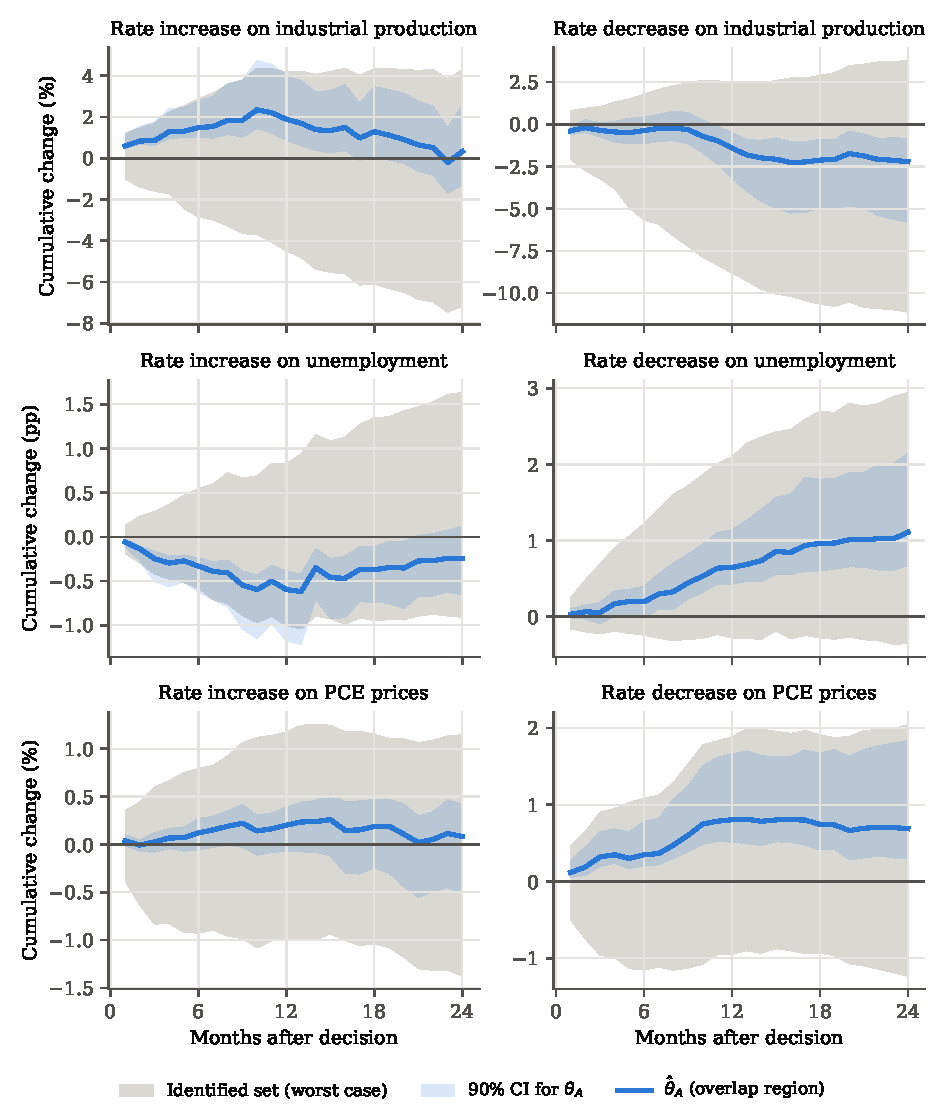
\includegraphics[width=0.92\linewidth]{responses_main.pdf}
  \caption{Cumulative effects of a rate increase (left) and decrease (right) relative to no change. Grey: worst-case
  identified set (Proposition~\ref{prop:bounds}). Blue: effect on the overlap region $\hat\theta^{\cA}_d$ with 90\%
  moving-block bootstrap interval. Greenbook propensity score; 133 meetings, 1989--2006.}\label{fig:responses}
\end{figure}

\paragraph{Worst-case bounds are not informative.} With $K$ equal to the range of outcomes the economy actually
experienced, every identified set contains zero at every horizon, and so does every \citet{imbens2004} interval.
Two years after a rate increase, the identified set for industrial production runs from $-7.2\%$ to $+4.3\%$. The
menus that exclude the action or the status quo account for a third or more of all meetings, and without an
assumption about them the data cannot sign the average effect. The 2020 version reported much narrower bounds
because it calibrated $K$ differently (Appendix~\ref{app:revision}).

\paragraph{The overlap-region effects have the wrong sign for real activity.} Where both the action and the status
quo were on the menu, the effects are point-identified and estimated with some precision. After a rate
\emph{increase}, industrial production is higher than under no change (by 1.5\% at six months and 1.9\% at twelve,
with 90\% intervals excluding zero through 18 months) and unemployment is lower (by 0.6 percentage points at twelve
months). After a rate \emph{decrease}, industrial production is lower by 1.4\% at twelve months and 2.2\% at
twenty-four, and unemployment is higher by 0.65 and 1.1 points. These are the opposite of the responses implied by
standard theory and found by most of the literature, and they are the same in the macro specification
(Appendix~\ref{app:robust}).

\paragraph{Staff forecasts remove the price puzzle.} The price responses behave differently. With the macro
information set, a rate increase is followed by significantly \emph{higher} prices from five months on, which is the
well-known price puzzle \citep{sims1992}. Conditioning on the Greenbook forecasts makes the price response to a rate increase
small and statistically indistinguishable from zero at every horizon (0.20\% at twelve months, interval
$[-0.07,0.39]$). This is the pattern \citet{romer2004} report: the puzzle reflects the Committee's reaction to
inflation it foresees, and the staff forecast captures that information. A rate decrease is followed by higher
prices under both specifications (0.8--1.0\% at twelve months), the direction theory predicts.

\begin{table}[!htbp]
  \centering
  \caption{Effects of rate changes relative to no change, Greenbook information set}\label{tab:results}
  \footnotesize
  \tablefile{results_main.tex}
  \par\medskip
  \begin{minipage}{0.86\linewidth}\footnotesize
  \emph{Notes:} Cumulative change $h$ months after the meeting. $\hat\theta_A$: effect on meetings whose menu contains
  both the action and no change, with basic moving-block bootstrap 90\% interval (499 draws, blocks of 8 meetings).
  Identified set: worst-case bounds on the average effect over all meetings (Proposition~\ref{prop:bounds}).
  $\lambda^\ast$: smallest heterogeneity between the non-overlap menus and the overlap region, in the outcome's
  units, that would make the sign of the average effect unidentified (Proposition~\ref{prop:lambda}).
  \end{minipage}
\end{table}

\paragraph{How much extrapolation is needed?} If effects were the same in every menu ($\lambda=0$), the
overlap-region estimates would be the average effects. The breakdown values in Table~\ref{tab:results} say how far
that homogeneity can be relaxed before the sign of the average effect is lost. For a rate increase, a third of the
meetings are outside the overlap region, so $\lambda^\ast=3\,|\hat\theta^{\cA}|$: the twelve-month IP response keeps its
sign unless the average effect in the menus without the status quo or without tightening differs from the
overlap-region effect by more than 5.7 percentage points. For a rate decrease two fifths of meetings lie outside the
region and $\lambda^\ast\approx2.4\,|\hat\theta^{\cA}|$. Figure~\ref{fig:sensitivity} traces the full set as a
function of $\lambda$. Reconciling the average effects with the textbook signs would require the effect in the
non-overlap menus to be not merely different from, but several times larger than and opposite in sign to, the effect
in the overlap region. That cannot be ruled out, but it would be an odd defence: the counter-theoretical signs come
from the meetings where the data are most informative, not from extrapolation.

\begin{figure}[!htbp]
  \centering
  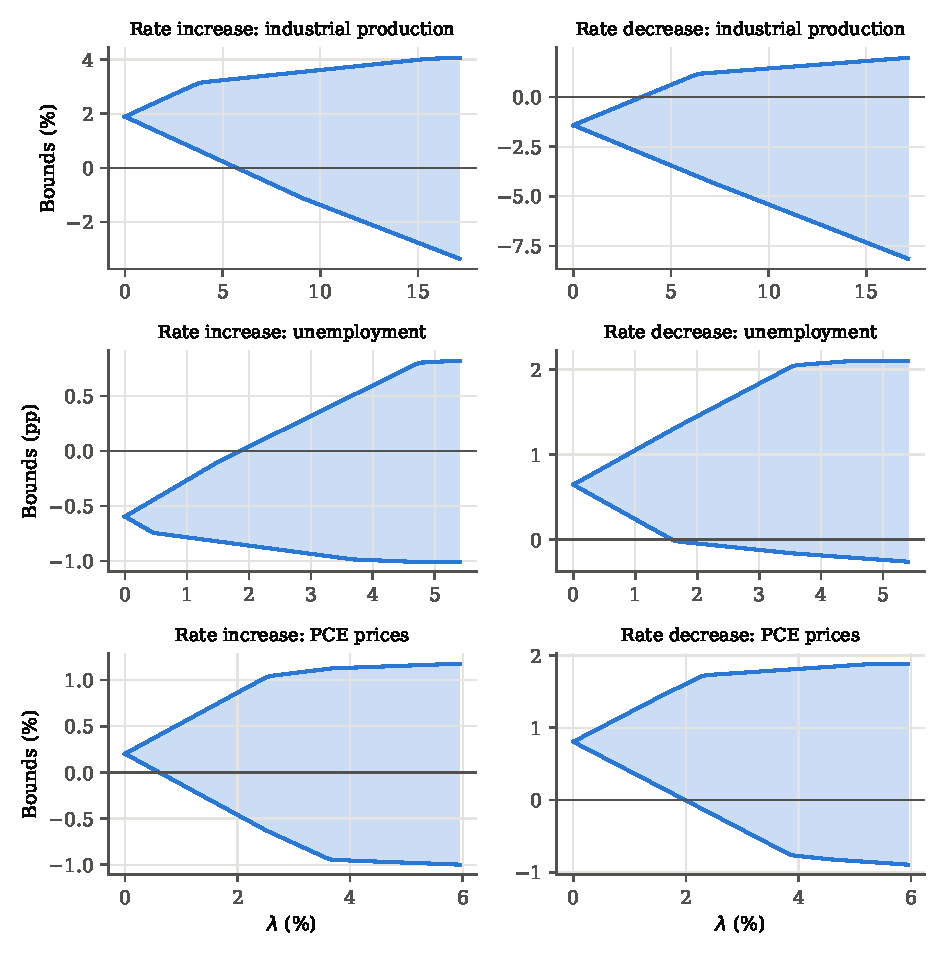
\includegraphics[width=0.86\linewidth]{sensitivity_main.pdf}
  \caption{Identified set for the twelve-month effect as a function of $\lambda$, the maximal difference between
  the average effect in a non-overlap menu and in the overlap region (Assumption~\ref{as:lambda}). At $\lambda=0$ the set is
  the point $\hat\theta^{\cA}_d$; for large $\lambda$ it reaches the worst case. Greenbook propensity score.}\label{fig:sensitivity}
\end{figure}

\paragraph{Interpretation.} The overlap-region estimates are credible only under Assumption~\ref{as:unconf}.
Their signs indicate that it fails. The Committee tightens when it expects the economy to strengthen, and
the expected strength shows up in subsequent output whether or not the Committee acts. Neither lagged data, market
expectations nor the Greenbook forecasts absorb this completely. Two features of the sample make the problem
hard to escape. First, the identifying variation is thin: all but one of the 27 tightenings come from $\{U,T\}$
menus, so the effect of a rate increase is essentially a comparison of hikes and holds within those 43 meetings.
Second, weighting within a menu only reweights meetings the Committee itself judged similar enough to offer the
same options, so the remaining differences between hikes and holds are exactly the judgemental information that
is hardest to measure. Asymmetries between increases and decreases, which the 2020 version emphasised following
\citet{hamilton2002} and \citet{angrist2011}, cannot be separated from this selection problem with the present
data.

\section{Discussion: The Results in Light of Recent Work}\label{sec:discussion}

Read against the literature of Section~\ref{sec:literature}, the results support three conclusions and point to
three extensions.

\paragraph{The counter-theoretical signs are the expected symptom of an incomplete information set.} The
overlap-region estimates imply that rate increases are followed by stronger activity. That is what one would see if
the Committee tightened when it had reason to expect strength that the econometrician's covariates do not capture.
This is the mechanism behind the information effect of \citet{nakamura2018} and, in the account of
\citet{bauer2023aer}, behind the predictability of market surprises by economic news. The finding that
Greenbook forecasts remove the price puzzle but not the real-activity puzzle fits the evidence in \citet{aruoba2025}
that the staff's written analysis contains information not summarised by its numerical forecasts. It also fits the
argument of \citet{romer2023} that isolating policy changes unrelated to the outlook requires reading the record,
not only conditioning on forecasts. The menus do not solve this problem, and they are not designed to. What they do
is separate it cleanly from the overlap problem, so that the remaining bias can be attributed to unconfoundedness.

\paragraph{The menu restriction is a genuine source of identifying information.} Imposing the menus raises the
likelihood of the decision model by as much as market expectations do, and it is exact rather than approximate.
Recent work that uses the same documents for other purposes \citep{doh2026,laarits2025} confirms that the Bluebook
alternatives are a well-defined and informative record of the Committee's deliberations. In the terms of the overlap
literature, the menus turn a problem of extreme estimated scores \citep{khan2010,heiler2021} into one of
structural zeros in a known region. That region can be handled by partial identification
\citep{susmann2025} instead of trimming, which would change the estimand.

\paragraph{Worst-case bounds alone are too wide for macroeconomic questions.} With one third to two fifths of
meetings outside the overlap region and outcome ranges that include the 2008--09 recession, the identified sets
contain zero everywhere. The same arithmetic makes the cross-sectional bounds of \citet{susmann2025} informative
only when the non-overlap subpopulation is small. In monetary policy it is not, so informative conclusions require
an additional assumption. The breakdown values $\lambda^\ast$ make that assumption explicit and give it units.

\paragraph{Extensions.} First, the menu-constrained propensity score can be combined with a richer information set.
Text-based measures of the staff's outlook in the spirit of \citet{aruoba2025} are the obvious candidate, and they
can be built from the same Bluebook and Greenbook corpus used here. Second, the $\lambda$-relaxation of effect
homogeneity can be paired with a relaxation of unconfoundedness along the lines of \citet{masten2018}. That would
report how much selection on unobservables is needed to overturn each sign, which is the question the results raise.
Third, the menus can be used with external shocks. \citet{kolesar2025} show that linear projections on an observed
shock identify a weighted average of causal effects even when the economy is nonlinear. Estimating such projections
within menus, with high-frequency surprises purged of prior news as in \citet{bauer2023nber}, would combine the
structural restriction documented here with a source of variation that does not rely on selection on observables.

\section{Conclusion}\label{sec:conclusion}

This thesis set out to relax one of the two assumptions behind semiparametric estimates of the effects of
monetary policy. Its central observation holds up: the Federal Reserve's own briefing documents show that some
actions are not on the table at some meetings, and the Committee never chose an action its staff had not
proposed. Treating the Bluebook menu as a covariate that dictates where the propensity score is zero gives a
decision model that fits markedly better at no cost in parameters, and a sharp characterisation of what the data
can and cannot say about the average effect of policy.

What the data can say is limited. Without restrictions on the menus that exclude the action or the status quo,
the average effect is not signed. With effects assumed similar across menus, the estimates are precise but have
the wrong sign for output and unemployment, even with the Greenbook forecasts in the propensity score. The
forecasts do remove the price puzzle for rate increases. The contribution of the menu is therefore to isolate the
problem. Overlap can be handled; unconfoundedness is what fails.

Section~\ref{sec:discussion} sets out the natural next steps: a richer, text-based information set inside the
menu-constrained propensity score, a sensitivity analysis for unconfoundedness alongside the one for effect
homogeneity, and the combination of the menu restriction with high-frequency policy surprises.


\bibliographystyle{plainnat}
\bibliography{references}

\appendix
\section{Proofs}\label{app:proofs}

\paragraph{Proof of Proposition~\ref{prop:bounds}.}
By the law of iterated expectations, $\theta_d=\sum_x\pi_x(\mu_d(x)-\mu_0(x))$, and $\pi_x$ is identified.

\emph{Identification of $\mu_a(x)$ for $a\in x$.} By Assumption~\ref{as:menu}, $p_a(x,z)>0$ for all $z$ in the
support of $Z\mid X=x$. By Assumption~\ref{as:unconf},
$\E[\1\{D=a\}Y\mid X=x,Z]=\E[\1\{D=a\}Y(a)\mid X=x,Z]=p_a(x,Z)\,\E[Y(a)\mid X=x,Z]$. Dividing by $p_a(x,Z)$ and
integrating over $Z\mid X=x$ gives \eqref{eq:ipw}.

\emph{Non-identification of $\mu_a(x)$ for $a\notin x$.} By Assumption~\ref{as:menu}, $\Prob(D=a\mid X=x)=0$, so
the distribution of observables $(Y,D,X,Z)$ places no restriction on the conditional distribution of $Y(a)$ given
$X=x$ beyond Assumption~\ref{as:bounded}. In particular, for any $m\in[K_1,K_2]$ the joint distribution
obtained by setting $Y(a)=m$ almost surely on $\{X=x\}$ generates the same observables, satisfies
Assumption~\ref{as:unconf} (a constant is independent of $D$), and has $\mu_a(x)=m$. Hence the identified set for
$\mu_a(x)$ is exactly $[K_1,K_2]$.

\emph{Sharpness of the sum.} The unidentified means $\{\mu_a(x): a\notin x\}$ enter $\theta_d$ linearly with
coefficients $\pm\pi_x$, and each can be set independently to either endpoint by the construction above, applied
menu by menu. The minimum of $\theta_d$ sets $\mu_d(x)=K_1$ for $x\in\cB_d\cup\cN_d$ and $\mu_0(x)=K_2$ for
$x\in\cC_d\cup\cN_d$; the maximum does the reverse. This gives $L_d$ and $U_d$. Every intermediate value is attained
by convex combination, so the identified set is the interval $[L_d,U_d]$. Subtracting yields the width. \qed

\paragraph{Proof of Proposition~\ref{prop:lambda}.}
Assumption~\ref{as:lambda} adds, for each $x\notin\cA_d$, the constraint
$\mu_d(x)-\mu_0(x)\in[\theta^{\cA}_d-\lambda,\theta^{\cA}_d+\lambda]$, where $\theta^{\cA}_d$ is identified. Intersecting with
the cell-level intervals of Proposition~\ref{prop:bounds} and summing gives the set. If no support constraint
binds, each cell contributes $\pi_x(\theta^{\cA}_d\pm\lambda)$, so the bounds are
$\pi(\cA_d)\theta^{\cA}_d+(1-\pi(\cA_d))(\theta^{\cA}_d\pm\lambda)=\theta^{\cA}_d\pm\lambda(1-\pi(\cA_d))$, which excludes zero iff
$\lambda<|\theta^{\cA}_d|/(1-\pi(\cA_d))$. \qed

\paragraph{Information in $X$ versus $Z$.}
If the menu contains all the information in $Z$ that predicts $D$, i.e.\ $p_a(x,z)=p_a(x)$, then
\eqref{eq:ipw} becomes $\mu_a(x)=\E[Y\mid D=a,X=x]$, a difference in means within menu, and conditioning on $Z$ is
harmless. In general
$\E[Y(a)\mid X=x]=\int\E[Y(a)\mid X=x,Z=z]\,dF_{Z\mid X=x}(z)$: the integral is over the distribution of $Z$
\emph{conditional on the menu}. The 2020 version integrated over the marginal distribution of $Z$, which is
incorrect when $X$ and $Z$ are dependent, as they are here.

\section{Robustness: macro information set}\label{app:robust}

Table~\ref{tab:results_alt} and Figure~\ref{fig:responses_alt} repeat the main results with the macro information
set of \citet{angrist2018} (column (3) of Table~\ref{tab:pscore}) in place of the Greenbook forecasts.

\begin{table}[p]
  \centering
  \caption{Effects of rate changes, macro information set}\label{tab:results_alt}
  \footnotesize
  \tablefile{results_alt.tex}
  \par\medskip
  \begin{minipage}{0.85\linewidth}\footnotesize
  \emph{Notes:} As Table~\ref{tab:results}, with the propensity score of Table~\ref{tab:pscore}, column (3).
  \end{minipage}
\end{table}

\begin{figure}[p]
  \centering
  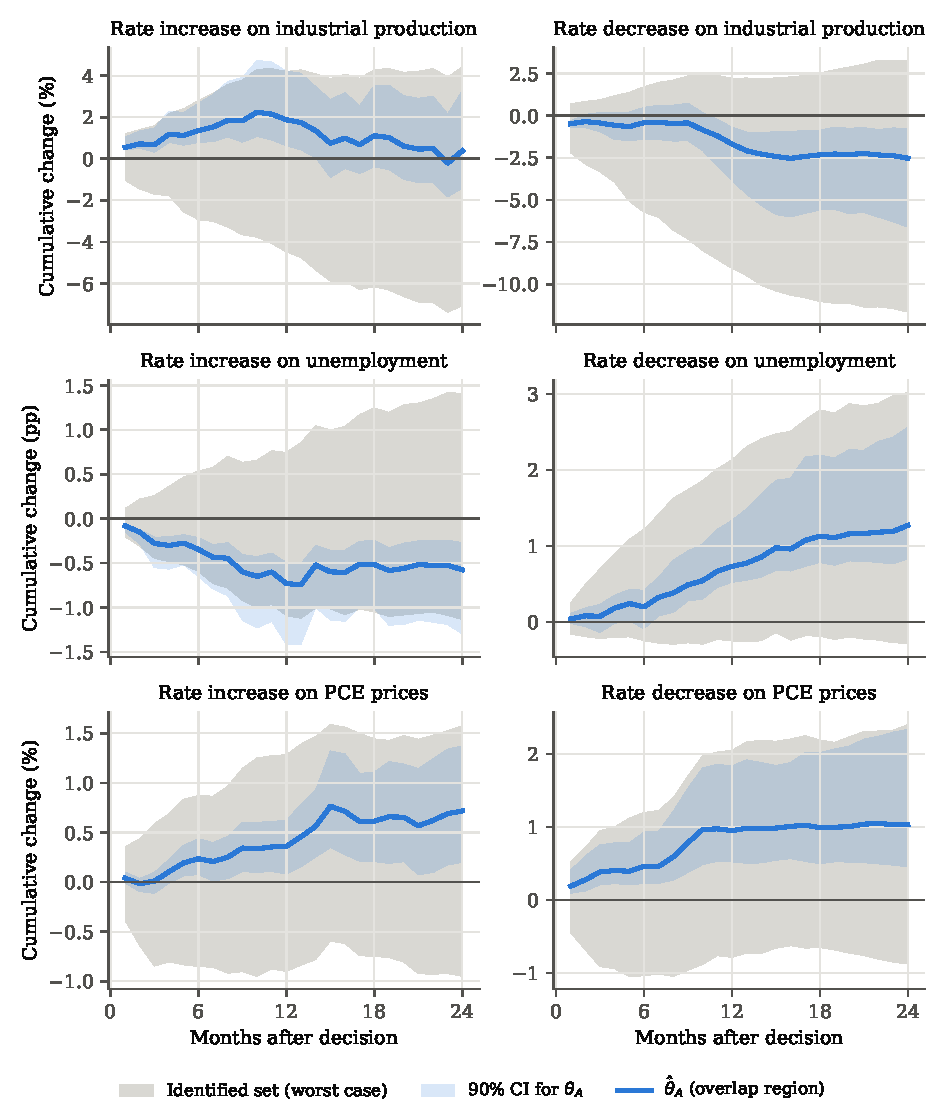
\includegraphics[width=0.92\linewidth]{responses_alt.pdf}
  \caption{Cumulative effects of rate changes, macro information set. See Figure~\ref{fig:responses}.}\label{fig:responses_alt}
\end{figure}

\section{Comparison with the 2020 version}\label{app:revision}

The revision changes the estimation in several ways, described in the main text: the propensity score now imposes
the menu's zeros and uses covariates observed at the time of the meeting (Section~\ref{sec:estimation}); the bounds
use the identified half of one-sided menus (Section~\ref{sec:framework}); the outcome bounds $K$ are calibrated to
the range of the outcome rather than to the spread of the estimates; cumulative effects are bounded directly; and
inference is reported. The 2020 estimation also applied a scaling step to the point-identified component of some
bounds that is not part of the estimator derived in Section~\ref{sec:framework}; the revision drops it. Most of the
difference in the real-activity results between the two versions comes from this step.


\end{document}
